\section{Local path planning}

Obstacle avoidance should follow the planned path and simultaneously avoid any unexpected obstacle that is not in the map.
There are several proposed methods in the literature, the main ones are: 
\begin{itemize}
    \item Potential field methods.
    \item Vector field histogram.
    \item Curvature-Velocity.
    \item Nearness diagram.
    \item Dynamic Window Approach.
\end{itemize}

\paragraph*{Bug-like robots}
Bug-like robots operate with limited knowledge: they are aware of the direction to the goal and possess local sensing capabilities for detecting obstacles using encoders.
Additionally, their world adheres to certain constraints: obstacles are finite within any finite range, and a line intersects an obstacle a finite number of times. 
The fundamental concept is to alternate between two primary behaviors:
\begin{enumerate}
    \item Directing toward the goal.
    \item Following obstacles until a clear path toward the goal is available again.
\end{enumerate}

\subsection{Vector Field Histograms}
Vector Field Histograms (VFH) utilize a local map of the environment to determine the optimal angle for driving. 
The environment is typically represented in a grid format (2 degrees of freedom) using local measurements, with all openings for the robot to pass through identified.
\begin{figure}[H]
    \centering
    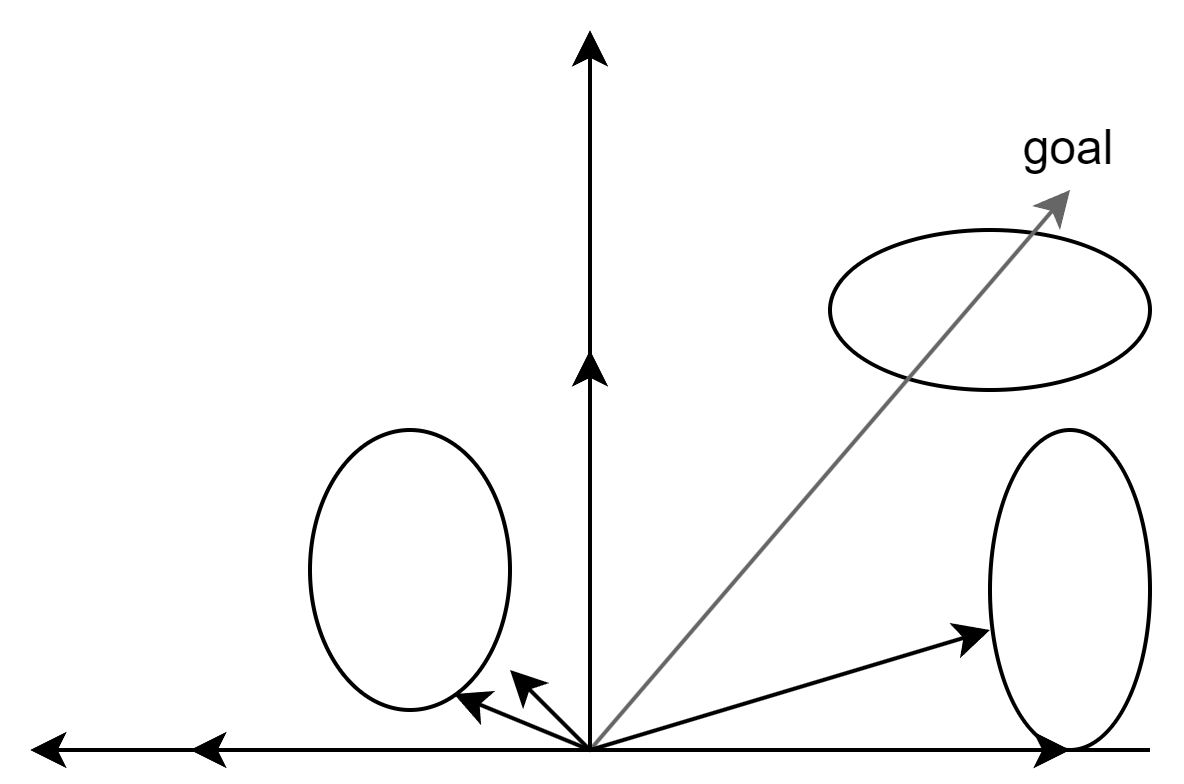
\includegraphics[width=0.5\linewidth]{images/vfh.png}
    \caption{Vector Field Histograms}
\end{figure}
To select the best angle for driving, a cost function needs to be defined and minimized:
\[G=a\cdot\text{target direction}+b\cdot\text{wheel orientation}+c\cdot\text{previous direction}\]
This function consists of three components:
\begin{itemize}
    \item $a\cdot\text{target direction}$ considers the alignment of the robot's path with the goal.
    \item $b\cdot\text{wheel orientation}$ accounts for the difference between the new direction and the current wheel orientation.
    \item $c\cdot\text{previous direction}$ takes into account the difference between the previously selected direction and the new direction.
\end{itemize}
The function computes the probability of hitting an obstacle and considers only the directions below a fixed threshold value. 
\begin{figure}[H]
    \centering
    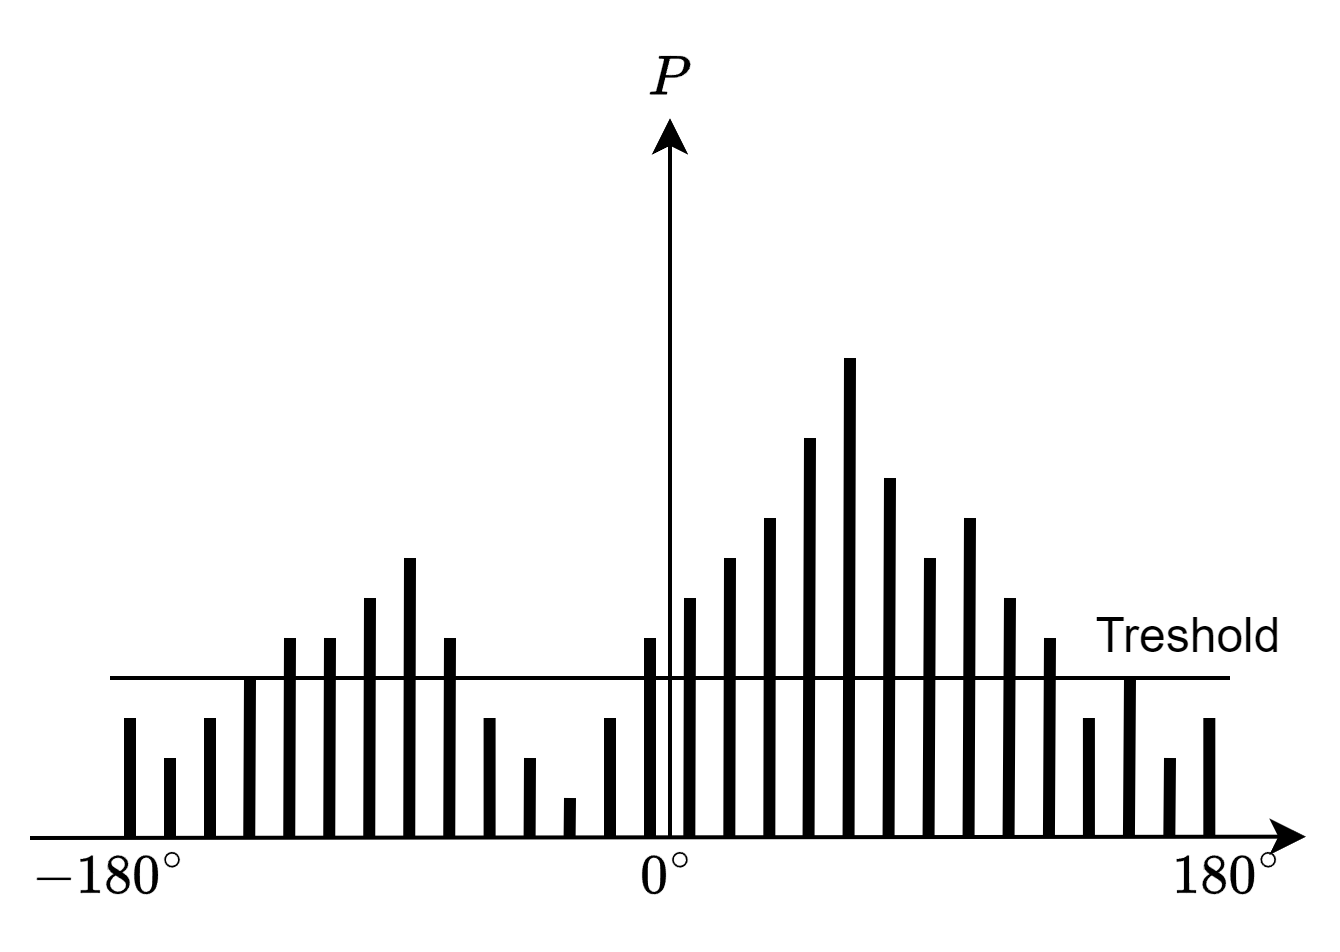
\includegraphics[width=0.5\linewidth]{images/fed1.png}
    \caption{Vector Field Histograms graph}
\end{figure}
This algorithm executes in constant time.

\subsection{Curvature Velocity Methods}
Curvature Velocity Methods incorporate physical constraints imposed by both the robot and the environment on the linear and angular velocities ($v,\omega$). 
These methods assume that the robot moves along arcs (where curvature $c=\frac{\omega}{v}$) with constraints on acceleration. 
Obstacles are transformed into velocity space, and an objective function is employed to select the optimal speed.

\subsection{Vector Field Histogram Plus}
VFH+ extends the capabilities of traditional VFH by incorporating vehicle kinematics. 
This includes considerations for a robot moving on arcs or straight lines. 
In VFH+, obstacles that block a particular direction impede all trajectories. 
Moreover, obstacles are enlarged to encompass all kinematically blocked trajectories.

\paragraph*{Limitations}
However, VFH+ shares some limitations with VFH:
\begin{itemize}
    \item Challenges arise when navigating through narrow areas like doors.
    \item Local minima might not be successfully avoided.
    \item There is no guarantee of reaching the goal.
    \item The dynamics of the robot are not fully considered.
\end{itemize}

\subsection{Dynamic Window Approach}
In the Dynamic Window Approach (DWA), the robot's kinematics are taken into account through a local search in velocity space.
This approach considers only circular trajectories represented by pairs of linear and angular speeds $V_s=(v,\omega)$. 
A velocity pair $V_a=(v,\omega)$ is deemed admissible if the robot can come to a stop before reaching the closest obstacle.
A dynamic window constrains the reachable velocities $V_d$ to those achievable within a short time frame given the robot's limited accelerations:
\[V_d=\begin{cases}
    v \in \left[v-a_{tr}\cdot t,v+a_{tr}\cdot t \right] \\
    \omega \in \left[\omega-a_{rot}\cdot t,\omega+a_{rot}\cdot t \right]
\end{cases}\]
Graphically, the scenario can be illustrated as follows:
\begin{figure}[H]
    \centering
    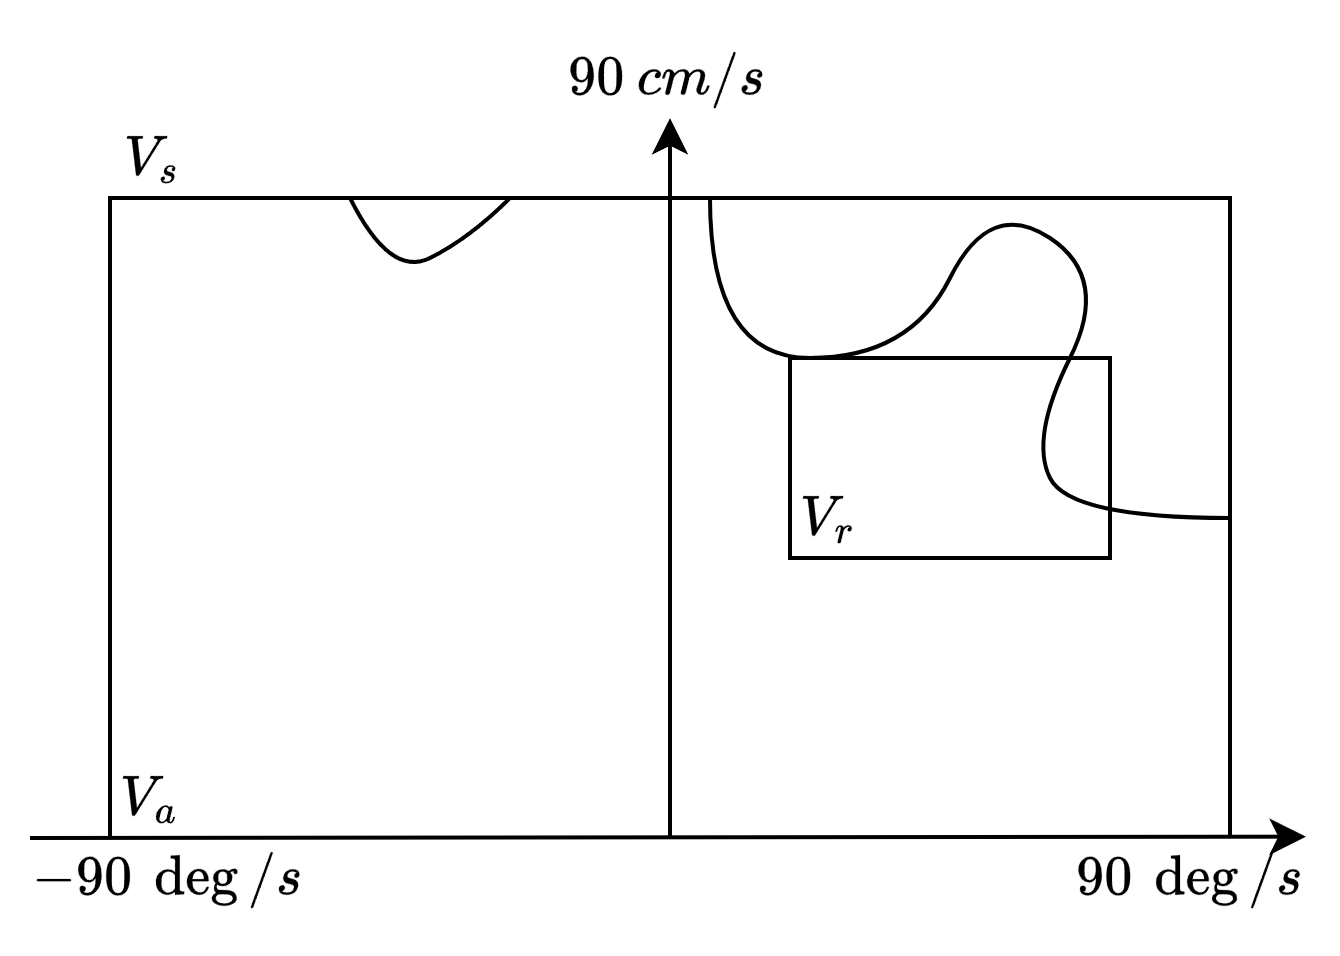
\includegraphics[width=0.6\linewidth]{images/dwa.png}
    \caption{Dynamic Window Approach search space}
\end{figure}
The objective is to find a feasible point within the search space defined as:
\[V_r =V_s \cap V_a \cap V_d\]

\paragraph*{Optimal combination}
The selection of the best pair $(v,\omega)$ is determined by maximizing a heuristic navigation function that minimizes travel time by driving quickly in the correct direction.
Planning is confined to the $V_r$ space, so the objective function is:
\[G(v,\omega)=\sigma\left(\alpha\cdot \text{heading}(v,\omega)+\beta\cdot\text{distance}(v,\omega)+\gamma\cdot \text{velocity}(v,\omega)\right)\]
Here, $\sigma(\cdot)$ is utilized because the function returns a probability. 
In this formulation:
\begin{itemize}
    \item $\alpha\cdot \text{heading}(v,\omega)$: considers alignment with the target direction.
    \item $\beta\cdot\text{distance}(v,\omega)$: considers the distance to the closest obstacle intersecting with curvature.
    \item $\gamma\cdot \text{velocity}(v,\omega)$: considers the forward velocity of the robot.
\end{itemize}

While this function provides local optimality, it may not be precise in selecting the best trajectory. 
To address this, a global approach using a navigation function in two-dimensional spaces can be employed:
\[\text{NF}=\alpha\cdot\text{velocity}+\beta\cdot\text{nf}+\gamma\cdot\Delta\text{nf}+\delta\cdot\text{goal}\]
Here:
\begin{itemize}
    \item $\alpha\cdot\text{velocity}$: considers the forward robot velocity.
    \item $\beta\cdot\text{nf}$: evaluates the cost to reach the goal.
    \item $\gamma\cdot\Delta\text{nf}$: assesses following the global path.
    \item $\delta\cdot\text{goal}$: takes into account the proximity to the goal.
\end{itemize}

\paragraph*{Dynamic Window Approach via trajectory rollout}
To estimate the trajectory, we employ the fundamental concept of the Dynamic Window Approach but with sampled control inputs. 
The process unfolds as follows:
\begin{enumerate}
    \item Discretely sample the robot's control space.
    \item For each sampled velocity, conduct a forward simulation to predict the outcome if applied for a short duration.
    \item Evaluate each trajectory resulting from the forward simulation.
    \item Discard illegal trajectories, namely those that intersect with obstacles, and select the trajectory with the highest score.
\end{enumerate}
This approach is versatile and can handle non-circular trajectories as well.
For instance, it can accommodate a clothoid, which is a trajectory characterized by a circular path with a radius that changes linearly.